\section{Optimizing Depthwise Convolution}
\label{sec:strategies} In this section, we describe our two optimizations, column reuse (Section \ref{sec:creuse}) and row reuse (Section
\ref{sec:rowreuse}), for reducing the number of GPU memory accesses for depthwise convolution.
\subsection{Column Reuse Optimization}
\label{sec:creuse}


\begin{figure}[t!]
\centering
  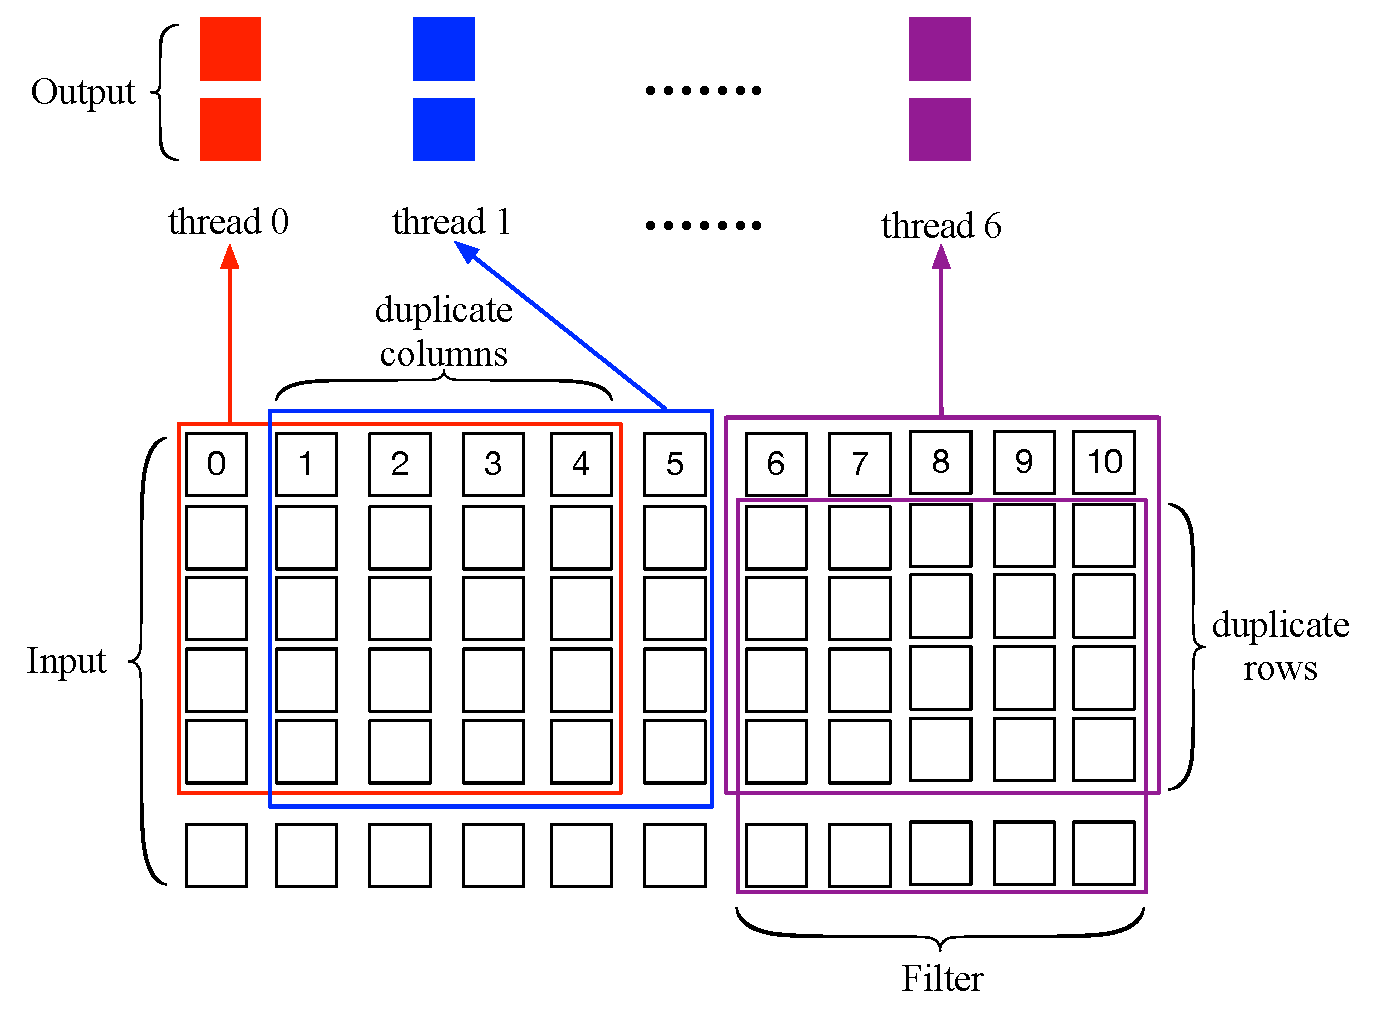
\includegraphics[width=0.9\columnwidth,height=5.5cm]{./figure/twostrategies.eps}
  \caption{Working example of performing a depthwise convolution using a GPU. Here, the filter size is $5 \times 5$, the input image size is $6 \times 11$
  and the output size is $2 \times 7$.}
  \label{fig:twostrategies}
\end{figure}


\mypara{Working example.} We use the depthwise convolution with only one channel shown in Figure \ref{fig:twostrategies} as a working
example to explain our column reuse method. In practice, we iterate the depthwise convolution kernel on each channel in turn (e.g., the R,
G, and B channels of an image). Without loss of generality, we slide a $5 \times 5$ filter over a $6 \times 11$ input with stride 1 to
produce a $2 \times 7$ output. Our column reuse method can also be applied to depthwise convolutions with other stride settings. In this
example, each thread calculates one column of the output. Two parallel threads 0 and 1 will execute code to slide the filter along the
width dimension, where both threads load two overlapped regions from the input image (thereby generating four duplicate columns).
Similarly, there will be another thread (thread 6 in this example) to slide the filter along the height dimension, which will load two
overlapped regions and generates four duplicate rows.


\begin{figure*}[!t]
\centering
\subfloat[Direct convolution: Each thread loads 5 input elements from global memory.]{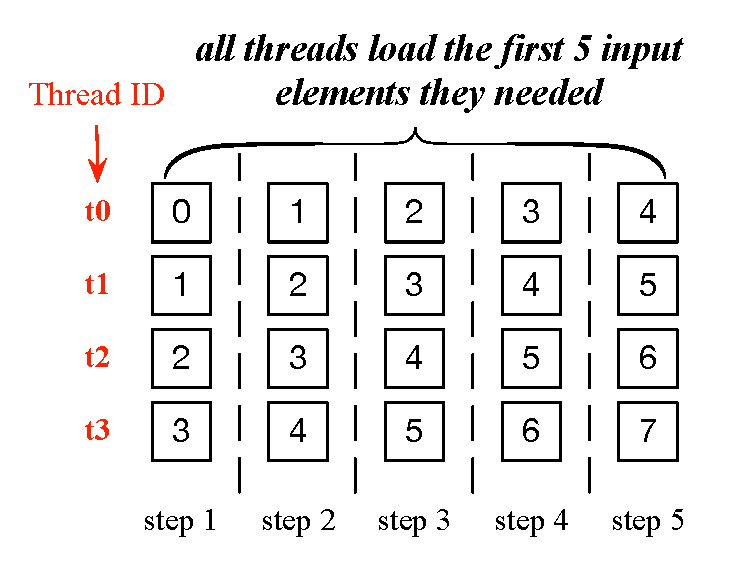
\includegraphics[width=0.3\textwidth,height=3.2cm]{./figure/directconv.eps}
	\label{fig:directalgo}}
\hspace{0em}
\subfloat[Optimized convolution: each thread retrieves its third element from the corresponding thread.]{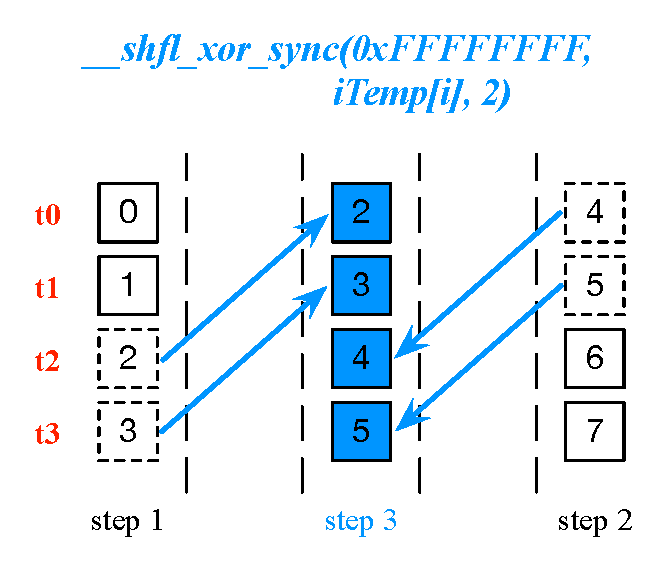
\includegraphics[width=0.3\textwidth,height=3.2cm]{./figure/optalgo1.eps}
	\label{fig:optalgo1}}
\hspace{0em}
\subfloat[Our approach: each thread retrieves its second and fourth elements from corresponding threads.]{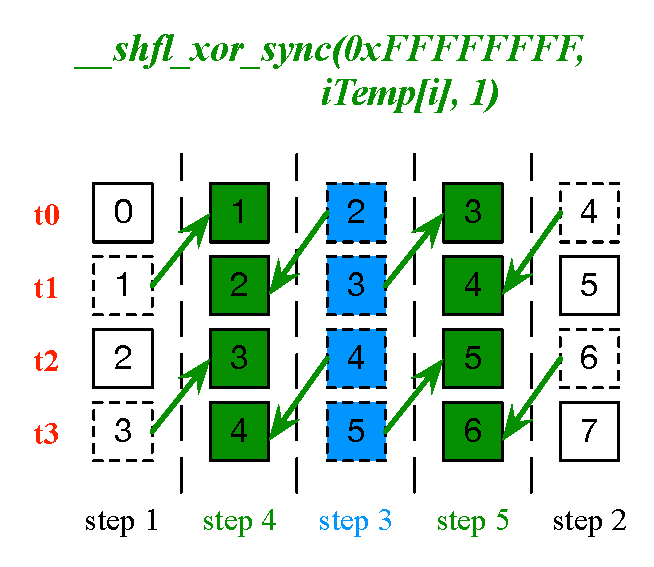
\includegraphics[width=0.3\textwidth,height=3.2cm]{./figure/optalgo2.eps}
	\label{fig:optalgo2}}

\caption{Illustration of direct and optimized convolutions. We use a $5 \times 5$ filter  and each thread calculates the convolution for
one output element. This example shows how a thread processes the first 5 corresponding input elements.} \label{fig:corealgo}
\end{figure*}
\subsubsection{Standard convolution} Figure \ref{fig:directalgo} shows a standard depthwise convolution operation, operating on a single-channel input on the example shown in Figure \ref{fig:twostrategies}.
Here, each thread loads the first corresponding input elements from the GPU global memory. Given that the indices of these elements are
contiguous, i.e., 0, 1, 2, and 3 in this example, concurrent access to these elements will be coalesced to form a single memory
transaction. As a result, each step will incur one memory access, five for the five steps (steps 1-5) as shown in Figure
\ref{fig:directalgo}. After completing step 5, each pair of adjacent threads will have four duplicate input elements, corresponding to the
duplicate columns in Figure \ref{fig:twostrategies}. Specifically, input elements 1, 2 and 3 loaded in step 2 would have already been
loaded by threads $t1$, $t2$ and $t3$ in the previous step (Figure \ref{fig:directalgo}). The repeated load to these elements leads to
redundant memory accesses and unnecessary memory access latency. Even the elements may be prefetched to the L1 cache before the next step,
access to the L1 cache still takes around 30 cycles on a 2080Ti GPU. To reduce the memory overhead, we would like to avoid such redundant
memory accesses.

\subsubsection{An optimized implementation} To eliminate the redundant loads, we could use the shuffle instructions supported by both CUDA and OpenCL to exchange input elements among
different threads. Figure \ref{fig:optalgo1} depicts such an optimization. Specifically, in steps 1 and 2 of Figure \ref{fig:optalgo1},
each thread loads the corresponding first and fifth input elements from the global memory. In step 3, each thread utilizes the shuffle
instruction to retrieve the third element from another thread. For example, threads $t0$ and $t1$ could retrieve the third element from
threads $t2$ and $t3$, respectively, and provide the fifth element (dashed squares in step 2) for both threads. Similarly, threads $t2$ and
$t3$ retrieve the third element from threads $t0$ and $t1$, respectively, and provide the first element (dashed squares in step 1) for
threads $t0$ and $t1$. Using the CUDA shuffle instruction, this exchange process can be implemented as $shfl\_xor(iTemp[i],2)$, where
$iTemp$ is a thread-local array used to store the five input elements, and $i$ is the location in the local array. For our working example,
threads $t0$ and $t1$ will supply the fifth element, hence $i=4$. Similarly, threads $t2$ and $t3$ will provide the first element, thus
$i=0$.

While this version reduces the redundant memory accesses compared to a standard convolution implementation, there is still room for improvement.
The problem is that the shuffle instruction $shfl\_xor(iTemp[i],2)$ now becomes a bottleneck because $iTemp$ is accessed through dynamic indexing.
Since the indices and the access pattern to $iTemp$ are not available at compile-time, the compiler cannot decide which of the elements in $iTemp$ will be frequently accessed and has to place $iTemp$ in the local memory which would still incur an access latency of around 500 cycles.
If we can promote register allocation for $iTemp$, we can then further improve the performance of convolution.

\subsubsection{Our approach}
Our column reuse approach (Figure \ref {fig:optalgo2}) thus converts dynamic indexing to static array access to promote register
allocation. This approach is described in Algorithms \ref{algo:basic} and \ref{algo:basic2}, where the first algorithm is used for step 3,
and the latter is used for steps 4 and 5. Note that these two algorithms can be used for different sized convolution kernels, for which we
will discuss in Section \ref {sec:rowreuse}.

Figure \ref{fig:exchange} shows the process of Algorithm \ref{algo:basic}. Here, we first load the corresponding first and fifth input
elements into $iTemp$ before passing it to Algorithm \ref{algo:basic}. Then, we pack two 32-bit elements into a 64-bit variable $exchange$,
where $iTemp[4]$ and $iTemp[0]$ are the high and low 32 bits, respectively (Line 2). As threads $t0$ and $t1$ will provide the fifth
element of the data they load, which are the high 32 bits of $exchange$, we right shift $exchange$ for both threads by an offset of 32 to
place $iTemp[4]$ in the low 32 bits. Now turning our attention to threads $t2$ and $t3$ that will provide the first element of the data
they loaded. Since the elements are the low 32 bits of $exchange$, we right shift $exchange$ in both threads by an offset of 0. The number
of places to be shifted for each thread is calculated based on the thread ID (Line 3). Next, we unpack $exchange$ into $iTemp[2]$ (high 32
bits) and $iTemp[1]$ (low 32 bits) (Line 5). By doing so, we can retrieve the element a thread needs to supply from a fixed location,
$iTemp[1]$. Finally, we use the shuffle instruction to exchange the elements among threads (Line 6).

\begin{algorithm}[t!]
\small

\tcp{$iTemp$: Buffer for storing input elements loaded from memory or generated through  \emph{shuffle} instructions.}
%\tcp{$iTemp$ contains input elements either loaded from global memory or through \emph{shuffle} instructions.}
\KwIn{$iTemp$}
	\KwOut{$iTemp$}
	$tid \gets threadIdx.x$\;
	$mov\ exchange, \{iTemp[0], iTemp[4]\}$\;
	$shift \gets ((tid+2)\&2)<<4$\;
	$exchange \gets exchange >> shift$\;
	$mov\ \{iTemp[1],iTemp[2]\}, exchange$\;
	$iTemp[2] \gets shfl\_xor(iTemp[1],2)$\;	
	
	\caption{RetrieveThirdElement}
	\label{algo:basic}
	
\end{algorithm}

Using Algorithm \ref{algo:basic}, we can replace the compile-time undecidable dynamic index $i$ in $shfl\_xor(iTemp[i],2)$ with static
indexing $1$ in $shfl\_xor(iTemp[1],2)$ of our working example. By doing so, we promote register allocation by allowing the compiler to put
all the thread-local variables into the fast GPU registers (that have access latency of 1 to 2 cycles as opposed to 500 cycles when the
data are stored in the local memory). Since steps 4 and 5 of our implementation (Figure \ref{fig:optalgo2}) adopt a similar procedure as
step 3 in Figure \ref{fig:optalgo1}, we can adapt Algorithm \ref{algo:basic} to obtain Algorithm \ref{algo:basic2} with minor
modifications. The main distinction between the two algorithms comes from how we process steps 3-5 shown in Figure \ref{fig:optalgo2}.
Specifically, we use four threads to exchange the elements in step 3 for Algorithm \ref{algo:basic}, but use only two adjacent threads in
steps 4 and 5 for Algorithm \ref{algo:basic2}. To adapt to the change of the number of threads used, we recalculate the shift offset for
each thread (Line 3 of both algorithms) and change the arguments of the shuffle instruction (Line 6 in both algorithms).

For our working example, Algorithms \ref{algo:basic} and \ref{algo:basic2} respectively reduce the number of memory accesses from 5 to 2
and 25 to 10 when 5 and 25 input elements are loaded. This reduction greatly improves the performance of the depthwise convolution.

\subsubsection{Generalize to other filter sizes} So far we have described our approach using a concrete working example with a pre-defined
filter size, but our algorithms can be generalized to filters with an arbitrary size. To apply our approach to a filter of size $n \times
n$, we will first divide the filter into several $n \times 5$ sub-filters. Next, we divide the remaining columns into several $n \times 3$
sub-filters with some overlap columns. For example, \FIXME{and as illustrated in Figure \ref{}}, a $7 \times 7$ filter can be divided into
a $7 \times 5$ sub-filter and a $7 \times 3$ sub-filter with one overlap column. Each $n \times 5$ and $n \times 3$ filters can then be
direcly processed by Algorithm \ref{algo:basic} and Algorithm \ref{algo:basic2}.


\begin{figure}[t!]
	\centering
	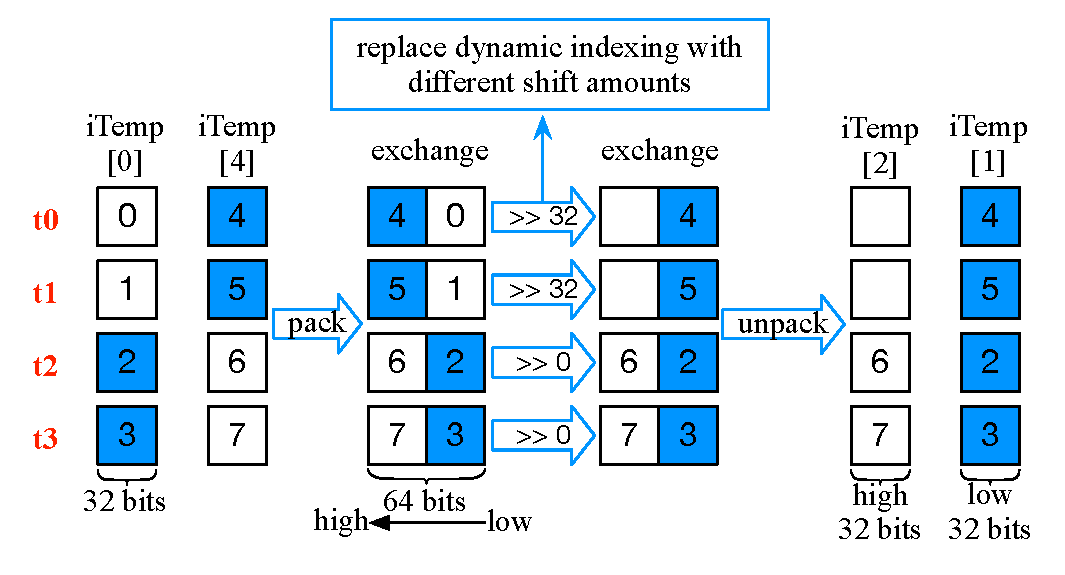
\includegraphics[width=0.8\columnwidth,height=3.5cm]{./figure/exchange.eps}
\caption{Convert dynamic indexing of array $iTemp$ into static indexing, allowing  $iTemp$ to be allocated in registers instead of the local memory.}
\label{fig:exchange}
\end{figure}

\begin{algorithm}[t!]
\small
	\KwIn{$iTemp$}
	\KwOut{$iTemp$}
	$tid \gets threadIdx.x$\;
	$mov\ exchange, \{iTemp[0], iTemp[2]\}$\;
	$shift \gets ((tid+1)\&1)<<5$\;
	$exchange \gets exchange >> shift$\;
	$mov\ \{iTemp[0],iTemp[1]\}, exchange$\;
	$iTemp[1] \gets shfl\_xor(iTemp[0],1)$\;	
	\caption{RetrieveSecondElement}
	\label{algo:basic2}
\end{algorithm}


\subsection{Row Reuse Optimization}
\label{sec:rowreuse}
\begin{figure}[t!]
	\centering
	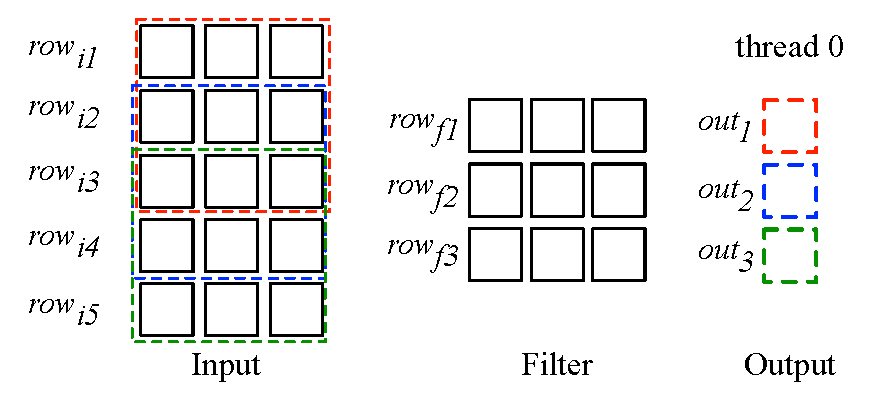
\includegraphics[width=0.8\columnwidth,height=3cm]{./figure/rowreuse.eps}
\caption{A $3 \times 3$ filter is used to slide over the input image along height dimension, which produces a column of output elements.}
\label{fig:rowreuse}
\end{figure}

\mypara{Working example.} Consider now the standard convolution example shown in Figure \ref{fig:rowreuse} as a working example for our row
reuse algorithm. When sliding the filter over the 2D input along the height dimension, it produces a column of elements as the output.

\subsubsection{Standard convolution} Assume we use one thread to calculate one column of output elements.
For the working example given in Figure \ref{fig:rowreuse}, the convolution will be computed as follows:
\begin{gather*}
  out_0=row_{i0} \cdot row_{f0} + row_{i1} \cdot row_{f1} + row_{i2} \cdot row_{f2} \\
out_{1}=row_{i1} \cdot row_{f0} + row_{i2} \cdot row_{f1} + row_{i3} \cdot row_{f2} \\
out_{2}=row_{i2} \cdot row_{f0} + row_{i3} \cdot row_{f1} + row_{i4} \cdot row_{f2}
\end{gather*}

As can be seen from the above equations, $row_{i1}$ and $row_{i3}$ are loaded twice, and $row_{i2}$ is loaded three times; nine rows are be
loaded in total. These redundant loads to the same read-only row thus incur extra memory accesses and additional overhead.

\subsubsection{Our optimization}
To remove redundant loads to the same row, we redesign the execution flow of the standard depthwise convolution. Specifically, after
fetching a row from the input, we compute the number of output elements that depend on the loaded row. For our working example, the
computation of element $out_0$ in the output column depends on $row_{i0}$. Similarly, output elements $out_0$ and $out_1$ will need
$row_{i1}$. With this information in place, we use the loaded row to perform inner products with corresponding rows of the filter to
calculate the output elements whose outcomes depending on the loaded row. Our approach translates the execution flow of the working example
presented in Figure \ref {fig:rowreuse} to:

\begin{equation}\nonumber
\begin{aligned}
load\ row_{i0}:
&\ out_0=row_{i0} \cdot row_{f0} \\
load\ row_{i1}:
&\ out_0 = out_0+row_{i1} \cdot row_{f1}\\
&\ out_1=row_{i1} \cdot row_{f0}\\
load\ row_{i2}:
&\ out_0 = out_0+row_{i2} \cdot row_{f2}\\
&\ out_1 = out_1+row_{i2} \cdot row_{f1}\\
&\ out_{2}=row_{i2} \cdot row_{f0}\\
load\ row_{i3}:
&\ out_1=out_1+row_{i3} \cdot row_{f2} \\
&\ out_2=out_2+row_{i3} \cdot row_{f1}\\
load\ row_{i4}:
&\ out_2=out_2+row_{i4} \cdot row_{f2}
\end{aligned}	
\end{equation}

In this new implementation, we would only issue loads to five rows to calculate the output elements of our working example. Compared to the
nine loads required by the standard convolution, we reduce the number of loads to row elements by nearly half. We note that although the
number of accesses to the output column $out$ is increased, the overhead is negligible because $out$ is smaller than the size of multiple
rows and often can be stored in registers.

We describe a general solution for row reuse in Algorithm \ref{algo:rowreuse}, where $row$ denotes the row loaded from the input, $index$ denotes the index of $row$, $filter$ denotes the vector of filter rows and $filter[i]$ means the $i$th row of the filter.
Pseudo code at Lines 1-5 process the first $F_H-1$ rows ($row_{i0}$ and $row_{i1}$ in Figure \ref{algo:rowreuse}) that are needed by less than $F_H$ output elements.
Code at lines 6-11 process the rows needed by exact $F_H$ output elements (e.g., $row_{i2}$ in Figure \ref{algo:rowreuse}).
Finally, code at Lines 12-17 process the last $F_H-1$ rows, which are needed by less than $F_H$ output elements (e.g., $row_{i3}$ and $row_{i4}$ in Figure \ref{algo:rowreuse}).

\begin{algorithm}[t!]
\small
	\KwIn{$row$, $index$, $filter$, $Out$}
	\KwOut{$Out$}
	\If{$index \textless F_H-1$}{
		\For {$i \gets 0$ \KwTo $index+1$}{
			$Out[i] \gets Out[i]+row \cdot filter[index-i]$\;
		}
	}\ElseIf{$index \geq F_H-1$ \textbf{and} $index \textless I_H-F_H+1$}{
		\For {$i \gets 0$ \KwTo $F_H$}{
			$o_{index} \gets index-F_H+1+i$\;
			$Out[o_{index}] \gets Out[o_{index}]+row \cdot filter[F_H-1-i]$\;
		}
	}\Else{
		\For {$i \gets F_H-1$ \KwTo $0$}{
			$o_{index} \gets I_H-F_H+1$\;
			$Out[o_{index}] \gets Out[o_{index}]+row \cdot filter[F_H-i]$\;
		}
	}
	\caption{RowReuse}
	\label{algo:rowreuse}
\end{algorithm}

Algorithm \ref{algo:rowreuse} is designed to eliminate redundant loads to the same row introduced by sliding a filter over the input along the height dimension.
By loading each row of the input just once, our approach greatly reduces the number of memory transactions for convolution operations.
